\documentclass[svgnames,tikz]{standalone}
\usetikzlibrary{positioning,backgrounds,calc}

\begin{document}
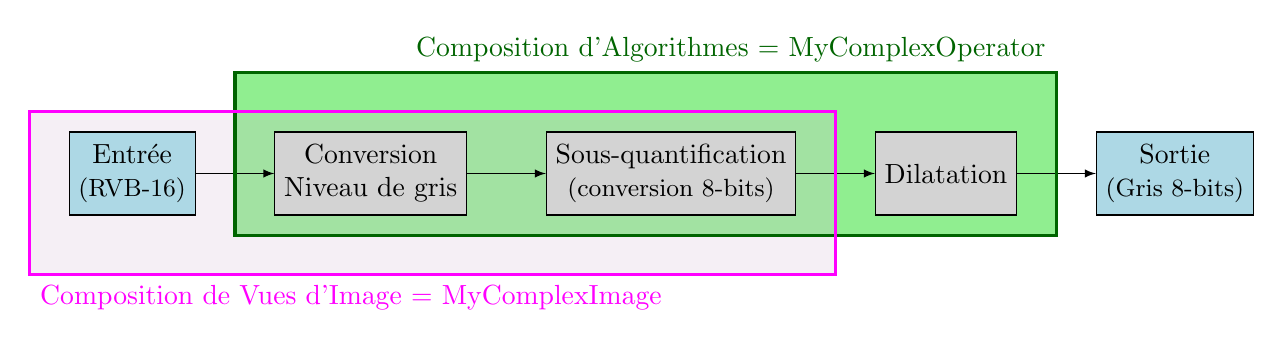
\begin{tikzpicture}
  \tikzset{
    Box/.style={draw, align=center, minimum height=30pt},
    ImageBox/.style={Box, fill=LightBlue},
    AlgoBox/.style={Box, fill=LightGrey}
  };


  \node[ImageBox] (A0) []            {Entrée\\ \small (RVB-16)};
  \node[AlgoBox]  (A1) [right=of A0] {Conversion\\Niveau de gris};
  \node[AlgoBox]  (A2) [right=of A1] {Sous-quantification\\ \small (conversion 8-bits)};
  \node[AlgoBox]  (A3) [right=of A2] {Dilatation};
  \node[ImageBox] (A4) [right=of A3] {Sortie\\ \small (Gris 8-bits)};

  \draw[-latex] (A0) -- (A1);
  \draw[-latex] (A1) -- (A2);
  \draw[-latex] (A2) -- (A3);
  \draw[-latex] (A3) -- (A4);

  %%\node [Olive, above=of A2] {Algorithm Composition};
  \draw[DarkGreen, very thick] ($ (A3.north east) + (.5,.75) $) node [DarkGreen, above left] {Composition d'Algorithmes = MyComplexOperator}
  rectangle ($ (A1.south west) + (-.5,-.25) $);


  \draw[Magenta, very thick] ($ (A0.south west) + (-.5,-.75) $) node [Magenta, below right] {Composition de Vues d'Image = MyComplexImage}
  rectangle ($ (A2.north east) + (.5,.25) $);

  \begin{scope}[on background layer]
    \fill[LightGreen] ($ (A1.north west) + (-.5,.75) $) rectangle ($ (A3.south east) + (.5,-.25) $);
    \fill[Thistle,opacity=0.25] ($ (A0.north west) + (-.5,.25) $) rectangle ($ (A2.south east) + (.5,-.75) $);
  \end{scope}


\end{tikzpicture}
\end{document}